\id{ҒТАМР 20.53.19}{}

\begin{articleheader}
\sectionwithauthors{С.З. Сапакова, Д. Даниярова, Н. Есмұхамедов, Р. Арманқызы, А.Б. Ембердиева, А. Қалдыбаева}{ДИАБЕТТІК РЕТИНОПАТИЯНЫ ЕМДЕУДЕ КӨЗ ТҮБІ ТІНДЕРІНЕ ЛАЗЕРЛІК ӘСЕРДІ МАТЕМАТИКАЛЫҚ МОДЕЛЬДЕУ}

{\bfseries
\textsuperscript{1}С.З. Сапакова\alink{https://orcid.org/0000-0001-6541-6806}\textsuperscript{\envelope },
\textsuperscript{2}Д. Даниярова\alink{https://orcid.org/0009-0000-5730-7407},
\textsuperscript{1}Н. Есмұхамедов\alink{https://orcid.org/0009-0006-0652-3082},
\textsuperscript{1}Р. Арманқызы\alink{https://orcid.org/0009-0009-2236-559X},
\textsuperscript{1}А.Б. Ембердиева\alink{https://orcid.org/0009-0005-5078-2412},
\textsuperscript{3}А. Қалдыбаева\alink{https://orcid.org/0000-0002-2062-182X}
}
\end{articleheader}

\begin{affiliation}
\textsuperscript{1}Халықаралық Ақпараттық Технологиялар Университеті, Алматы, Қазақстан,

\textsuperscript{2}Халықаралық білім беру корпорациясы, Алматы, Қазақстан,

\textsuperscript{3}Қазақ ұлттық қыздар педагогикалық университеті, Алматы, Қазақстан

\raggedright \textsuperscript{\envelope }Корреспондент-автор: sapakovasz@gmail.com
\end{affiliation}

Бұл жұмыс диабеттік ретинопатияны емдеуде лазерлік терапияны
оңтайландыру мақсатында көз\-дің түбі тіндеріне лазерлік әсерді
математикалық модельдеуге арналған. Мақалада тіндердегі температураның
таралуын модельдеу әдістері және лазердің параметрлерін пайдалана
отырып, көз торына (сетчаткаға) тиімді әсер ету жолдары қарастырылады.
Зерттеу барысында лазерлік әсер кезінде жылу өткізгіштігін сипаттайтын
дифференциалды теңдеулер және жылу әсерлерін болжауға арналған арнайы
математикалық модельдер қолданылды. Моделдер лазерлік энергияның терең
тіндерге таралуын, сонымен қатар лазердің әсерін бақылауды
оңтайландыруды қамтамасыз етеді. Зерттеуде уақыт пен тереңдік бойынша
температураның таралуын модельдеуге ерекше көңіл бөлінді, бұл лазердің
параметрлерін (қуаты, импульс ұзақтығы, қарқындылығы) дәл баптауға
мүмкіндік береді. Моделдеу нәтижелері тіндердің беткі қабаттарында
температураның айтарлықтай тез көтерілуі және терең қабаттарда баяу
таралуы байқалғанын көрсетті, бұл лазерлік әсерді дәл бақылаудың
маңыздылығын растайды. Мақалада көз ауруларын емдеуде лазердің
параметрлерін дұрыс таңдаудың маңыздылығы талқыланады, әсіресе диабеттік
ретинопатияны емдеуде. Ұсынылған модельдер офтальмологиядағы лазерлік
технологияларды әрі қарай дамытуға және лазерлік терапияның қауіпсіздігі
мен тиімділігін арттыруға мүмкіндік береді. Сонымен қатар, лазерлік
әсерді тиімді қолдану үшін қосымша зерттеулер мен эксперименттер қажет
екені көрсетілген.

{\bfseries Түйін сөздер:} лазерлік терапия, диабеттік ретинопатия,
математикалық модельдеу, температура, лазер параметрлері,
дифференциалдық теңдеулер.

\begin{articleheader}
{\bfseries МАТЕМАТИЧЕСКОЕ МОДЕЛИРОВАНИЕ ЛАЗЕРНОГО ВОЗДЕЙСТВИЯ НА ГЛАЗНОЕ ДНО ПРИ ЛЕЧЕНИИ ДИАБЕТИЧЕСКОЙ РЕТИНОПАТИИ}

{\bfseries
\textsuperscript{1}С.З. Сапакова\textsuperscript{\envelope },
\textsuperscript{2}Д. Даниярова,
\textsuperscript{1}Н. Есмұхамедов,
\textsuperscript{1}Р. Арманқызы,
\textsuperscript{1}А.Б. Ембердиева,
\textsuperscript{3}А. Қалдыбаева
}
\end{articleheader}

\begin{affiliation}
\textsuperscript{1} Международный университет информационных технологий, Алматы, Казахстан

\textsuperscript{2} Международная образовательная корпорация, Алматы, Казахстан,

\textsuperscript{3} Казахский национальный женский педагогический университет, Алматы, Казахстан,

e-mail: sapakovasz@gmail.com
\end{affiliation}

Данная работа посвящена математическому моделированию лазерного
воздействия на ткани глазного дна с целью оптимизации лазерной терапии
при лечении диабетической ретинопатии. В статье рассматриваются методы
моделирования распределения температуры в тканях и способы эффективного
воздействия на сетчатку с использованием лазерных параметров. В процессе
исследования применялись дифференциальные уравнения, описывающие
теплопроводность, а также специальные математические модели для
прогнозирования тепловых эффектов при лазерном воздействии. Модели
обеспечивают оптимизацию распространения лазерной энергии в глубокие
такни и контроль воздействия лазера. Особое внимание уделено
моделированию распределения температуры во времени и по глубине, что
позволяет точно настроить параметры лазеры (мощность, продолжительность
импульса, интенсивность). Результаты моделирования показали, что
температура в поверхностных слоях повышается значительно быстрее, чем в
глубоких, что подтверждает необходимость точного контроля лазерного
воздействия. В статье обсуждается важность правильного выбора лазерных
параметров для лечения глазных заболеваний, особенно диабетической
ретинопатии. Предложенные модели могут способствовать дальнейшему
развитию лазерных технологий в офтальмологии и улучшению безопасности и
эффективности лазерной терапии. Также указано, что для эффективного
применения лазерного воздействия необходимы дополнительные исследования
и эксперименты.

{\bfseries Ключевые слова:} лазерная терапия, диабетическая ретинопатия,
математическое моделирование, температура, лазерные параметры,
дифференциальные уравнения.

\begin{articleheader}
{\bfseries MATHEMATICAL MODELING OF LASER EXPOSURE ON THE FUNDUS IN THE
TREATMENT OF DIABETIC RETINOPATHY}

{\bfseries
\textsuperscript{1}S.Z. Sapakova\textsuperscript{\envelope },
\textsuperscript{2}D. Daniyarova,
\textsuperscript{1}N. Yesmukhamedov,
\textsuperscript{1}R. Armankyzy,
\textsuperscript{1}A.B. Emberdieva,
\textsuperscript{3}A. Kaldybaeva
}
\end{articleheader}

\begin{affiliation}
\textsuperscript{1} International University of Information Technologies, Almaty, Kazakhstan,

\textsuperscript{2} International Educational Corporation, Almaty, Kazakhstan,

\textsuperscript{3} Kazakh National Women' s Pedagogical University, Almaty, Kazakhstan,

e-mail: sapakovasz@gmail.com
\end{affiliation}

This paper is dedicated to the mathematical modeling of laser exposure
on the fundus tissues for optimiz\-ing laser therapy in the treatment of
diabetic retinopathy. The article discusses methods of modeling the
distribution of temperature in tissues and ways to effectively impact
the retina using laser parameters. Differential equations describing
heat conduction and specialized mathematical models for predicting
thermal effects during laser exposure were used in the study. The models
ensure the optimization of laser energy distribution to deep tissues and
control of laser effects. Special attention was paid to modeling the
temperature distribution over time and depth, which allows for the
precise adjustment of laser parameters (power, pulse duration,
intensity). The modeling results showed that the temperature in surface
layers increases significantly faster than in deeper layers, confirming
the importance of precise laser impact control. The paper discusses the
importance of choosing the correct laser parameters in the treatment of
eye diseases, especially diabetic retinopathy. The proposed models can
contribute to the further development of laser technologies in
ophthalmology and enhance the safety and effectiveness of laser therapy.
Additionally, it is noted that further research and experiments are
required for the effective application of laser exposure.

{\bfseries Keywords:} laser therapy, diabetic retinopathy, mathematical
modeling, temperature, laser parameters, differential equations.

\begin{multicols}{2}
{\bfseries Кіріспе.} Диабеттік ретинопатия -- бұл қант диабетінің ұзаққа
созылған ағымына байланысты дамитын көздің ретиналды ауруы. Глюкоза
алмасуының бұзылуы салдарынан көздің тор қабығын қоректендіретін қан
тамырлары зақымданып, көрудің нашарлауына әкеледі және уақытында
емделмеген жағдайда соқырлыққа себеп болуы мүмкін. Лазерлік терапия
диабеттік ретинопатияны емдеудің тиімді әдістерінің бірі болып табылады,
ол тор қабығының зақымдануын болдырмауға және оның одан әрі дамуын
тоқтатуға бағытталған. Лазерлік сәулелену тор қабығына әсер етіп,
ақуыздардың коагуляциясын және аномальды тамырлардың жойылуын тудырады,
бұл аурудың дамуын тоқтатуға көмектеседі. Дегенмен, лазерлік
технологияларды офтальмологияда тиімді пайдалану үшін лазерлік
сәулеленудің тор қабығына әсерін дәл моделдеу қажет. Лазерлік коагуляция
жергілікті температураның көтерілуіне әкеледі, бұл зақымданған және сау
тіндерге зиян келтіруі мүмкін, егер лазердің параметрлері дұрыс
таңдалмаса. Лазерлік сәуленің тиімділігін модельдеу үшін көз тіндерінің
бірнеше қасиеттерін, оның ішінде олардың біртекті еместігін, лазерлік
сәулеленумен жылу процесін, лазердің параметрлерін (толқын ұзындығы,
қуат, импульс ұзақтығы және жиілік) және тор қабығы мен қоршаған
тіндердің биомеханикалық қасиеттерін ескеру қажет. Лазерлік сәулеленудің
көз түбіне әсерін математикалық моделі көптеген факторлардың әсерін
ескеру қажет болғандықтан күрделі болып табылады. Әрбір жаңа модель
лазерлік сәуленің тор қабығына әсерін дәл болжауға және оны емдеу үшін
ең тиімді параметрлерді таңдауға мүмкіндік береді. Қазіргі уақытта
математикалық модельдер лазерлік сәулеленудің көз тіндеріне әсерін
болжауға және лазердің параметрлерін оңтайландыруға көмектеседі.
Модельдер тіндердің құрылымын, температураның таралуын және лазерлік
энергияның әсерін ескеріп, лазердің әсер ету шекараларын анықтауға
бағытталуы тиіс.

Бұл зерттеудің мақсаты -- лазерлік коагуляцияның тор қабығына әсерін
сипаттайтын математикалық модельді құру, сондай-ақ лазердің әртүрлі
параметрлерінің диабеттік ретинопатияны емдеудегі тиімділігіне әсерін
зерттеу.

Зерттеу міндеттері: лазерлік сәулеленудің тор қабығына әсерін сипаттау,
жылу процестерін ескеру, лазердің параметрлерін талдау және олардың
әсерін тексеру, сондай-ақ зақымданудың азаюы үшін бұл параметрлерді
оңтайландыру. Бұл мақсаттарға жету үшін математикалық модельдеу және
жылу процестерін есептеу үшін сандық әдістер қолданылады.

Зерттеу гипотезасы -- лазерлік сәулеленудің әсерін дәл модельдеу, барлық
параметрлер мен көз тіндерінің ерекшеліктерін ескере отырып, лазерлік
терапияның қауіпсіздігін арттырып, оның тиімділігін жақсартуға мүмкіндік
береді. Зерттеудің теориялық маңызы -- лазерлік терапияны математикалық
модельдеудің жаңа тәсілдерін дамыту, ал практикалық маңызы -- лазердің
параметрлерін оңтайландыру және офтальмологиялық процедуралардың
қауіпсіздігін арттыруға құралдарды дамыту.

Қазіргі уақытта лазерлік терапия офтальмология саласында маңызды әдіс
болып табылады, әсіресе диабеттік ретонопатия мен макулярды ісіну сияқты
көз ауруларын емдеуде. Лазерлік сәулеленудің әсерін дәл модельдеу
лазерлік фотокоагуляция мен басқа да лазерлік емдеу әдістерінің
тиімділігі мен қауіпсіздігін арттыруға көмектеседі. Бұл зерттеулер
лазерлік сәулеленудің тор қабығына термикалық әсерін зерттеуге және оның
нәтижелерін болжауға бағытталған. Мысалы, авторлар оптикалық когерентті
томография арқылы көз түбінің үш өлшемді құрылымын қалпына келтіріп, тор
қабығын сегментациялау мен лазерлік әсерді модельдеудің алгоритмдерін
ұсынған. Бұл модель түрлі лазерлер мен лазерлік сәулеленудің әсері
бойынша коагуляцияның өлшемдерін, сондай-ақ зақымдану шекараларын
болжауға мүмкіндік береді. Модельдің нәтижелері интервалдардың саны екі
еселенгенде орташа квадраттық ауытқу 1,7-5,9 есе төмендегенін көрсетті,
бұл лазерлік терапияның тиімділігі мен қауіпсіздігін арттырып, оның
негізгі параметрлерін бағалауға мүмкіндік береді {[}1{]}. Сонымен қатар,
лазерлік сәулеленудің биологиялық тіндерге әсерін модельдеу маңызды
мәселе болып табылады. MILI моделін қолдану арқылы лазер сәулеленуінің
оңтайлы параметрлері, энергияның сіңірілуі, жылудың таралуы және
тіндердің өзгерістері есептеледі. Бұл моделдеу тіндердің лазерлік
сәулеленуге реакциясын болжауға және тіндердің қызып кету қаупін
бағалауға мүмкіндік береді, яғни лазерлік терапияның қауіпсіз әрі тиімді
болуына ықпал етеді {[}2{]}. Лазер мен тіндердің өзара әрекеттесу
механизмдерін сандық талдау лазерлік операциялардың тиімділігін
арттыруда маңызды рөл атқарады. Осы мақсатта, көпқабатты біртекті орта
моделін қолдана отырып, лазерлік сәуленің таралуы мен энергияны сіңіруді
модельдеу үшін көпқабатты Монте-Карло әдісі қолданылған. Бұл модельдің
нәтижелері фототермальды әсерлер мен жылулық зақымдануды лазер
сәулесінің белгілі параметрлеріне байланысты анықтауға мүмкіндік береді.
Бұл зерттеу лазерлік терапияның тиімділігін арттыру үшін маңызды болып
табылады, әсіресе клиникалық нәтижелерді жақсартуға бағытталған {[}3{]}.
Жасушалық деңгейде лазерлік сәулеленудің тор қабығына термикалық зақым
келтіретін энергияны есептеу үшін арнайы компьютерлік модельдер жасалды.
Модельдің нәтижелері эксперименттік деректермен салыстырылғанда 31\%
ауытқумен жақсы сәйкес келді, бұл лазерлік өнімдердің қауіпсіздігін
қамтамасыз ету үшін қажетті ғылыми негіздер болып табылады. Осы
модельдер лазерлік өнімдердің тәуекелдерін бағалауға және тор қабығының
зақымдану шегін болжауға мүмкіндік береді {[}4{]}. Көз түбінің
температуралық өзгерістерін зерттеу барысында түрлі лазерлер мен олардың
әсер ету режимдерін қолдана отырып, жаңа модельдер ұсынылды. Бұл
модельдер лазерлік сәулеленудің биологиялық тіндерге әсерін алдын-ала
болжауға мүмкіндік береді және лазерлік абляция мен фотодисрупцияның
нәтижелерін бағалауға көмектеседі. Лазерлік сәулеленудің әсерінен
тіндердегі жылулық зақымдану шегін болжау үшін фототермальды және
фотохимиялық процестерді in vitro моделінде ажырату қажеттілігі
айтылады. Бұл үшін Аррениустың бірінші ретті жылдамдық тұрақтысы мен
интегралы қолданылады {[}5{]}. Лазерлік фотокоагуляция әдісінің
тиімділігін арттыру үшін лазер сәулесінің параметрлерін дәл есептеу өте
маңызды. Model Predictive Control (MPC) әдісі лазерлік сәулеленудің жылу
теңдеуін шешуді қажет етеді, бұл лазердің сәулелену ұзындығы, уақыты мен
энергияның таралу профилі сияқты параметрлердің температураға әсерін
бағалауға мүмкіндік береді. Бұл әдіс лазердің қауіпсіздігін арттырып,
лазерлік терапияның тиімділігін жоғарылатуға көмектеседі {[}6{]}.
Зерттеулер көрсеткендей, температураның көтерілуіне сезімталдық жоғары,
әсіресе пигментті эпителийдің сіңіру коэффициентіне қатысты {[}7{]}.
Лазерлік сәулеленудің көз түбіне әсерін түсіну, оның зақымдану шектерін
болжауға және лазерлік офтальмохирургиядағы жаңа әдістерді әзірлеуге
ықпал етеді. Пеннеспила био-жылу теңдеуі негізіндегі модельдер лазерлік
сәулелену мен тіндердің өзара әрекеттесуін зерттеуге мүмкіндік береді
және клиникалық нәтижелерді бағалауға ықпал етеді {[}8{]}. Бұл модельдер
лазерлік терапияның қауіпсіздігін арттыруға және жаңа лазерлік
технологияларды клиникалық тәжірибеге енгізуге көмектеседі. Қорытындылай
келе, лазерлік сәулеленудің көз түбіне термикалық әсерін модельдеу өте
маңызды қадам болып табылады, себебі бұл зерттеулер лазерлік терапияны
тиімдірек және қауіпсіз ету үшін қажетті ғылыми негіздерді қамтамасыз
етеді. Моделдеу нәтижелері лазерлік сәулеленудің көз тіндеріне әсерін
дәл болжауға мүмкіндік береді, бұл лазерлік терапия әдістерін
жетілдіруге жол ашады {[}9{]}. Лазерлік сәулеленудің көз түбіне әсерін
зерттеу бойынша соңғы зерттеу 10 нс-тан 1 с-қа дейінгі сәулелену
импульстарының әсерін талдайды. Бұл зерттеу лазерлік офтальмохирургия
үшін негізгі физикалық процестерді математикалық модельдеу мен зерттеу
нәтижелерін ұсынады. Модель түрлі лазерлер мен олардың әсер ету
режимдері үшін коагуляцияның салыстырмалы өлшемдері мен зақымдану
шекараларын генерациялайды. Сондай-ақ, көз ауруларын емдеу мен диагноз
қоюға арналған нақты қолданбаларды ұсынады {[}10{]}. Келесі жұмыста
авторлар лазерлік сәулеленудің адам көзінде жылулық әсерін модельдеуге
арналған бұрын жарияланған жұмысқа кеңейту болып табылады.2D модель
3D-ге кеңейтілді, бұл көздің лазермен сәулеленуін нақтырақ бейнелеуге
мүмкіндік береді. Модель Пеннес био-жылу өткізгіштігі теңдеуімен
жасалып, шектеулі элементтер әдісімен шешіледі, Галеркин-Бубнов
процедурасы қолданылған. Көз ішіндегі температуралық өріс үшін алынған
нәтижелер офтальмологиялық процедуралар кезінде көз ішіндегі тіндерге
болатын зақымдануларды минимизациялауға пайдалы болуы мүмкін, сондай-ақ
лазер мен тіндердің өзара әрекеттесу механизмдерін талдауда да пайдалы
болады {[}11{]}. Авторлар зерттеулерін лазерлік сәулеленудің көзге
әсерінен болатын жылулық зақымдануды болжау моделін тексеруге арнаған.
Модель төрт кезеңнен тұрады: лазерлік бейненің тор қабығында есептелуі,
көз тіндерінде пайда болатын жылудың есептелуі, температураның көтерілуі
және зақымдану шегін анықтау. Техас университеті модельді тексеру үшін
клеткалармен және жануарлармен тәжірибелер жүргізді. Тәжірибелерде түрлі
лазерлік әсерлерге байланысты интенсивтілік, температура, шекті қуат
және зақымдану дәрежесі өлшенді {[}12{]}.

{\bfseries Материалдар мен әдістер.} Көз түбіне лазерлік әсерді модельдеу
үшін қолданылатын негізгі математикалық модельдер, лазерлік сәулеленудің
көз тіндеріне әсерін болжауға және осы әсердің жылу процестерін дәл
сипаттауға мүмкіндік береді. Бұл модельдер әртүрлі факторларды, оның
ішінде лазердің параметрлерін, көз тіндерінің қасиеттерін және
биомеханикалық ерекшеліктерін ескереді. Төменде осы модельдердің негізгі
түрлері мен олардың құрылымы қарастырылған. Лазерлік сәулелену көздің
тор қабығына әсер етіп, оның жылулық өзгерістеріне әкеледі. Бұл
әсерлердің барлық аспектілерін сипаттау үшін әртүрлі физикалық
процестерді біріктіретін математикалық модельдер қажет. Модельдер
негізінен лазерлік сәулеленудің тіндерге өтуін және лазердің әсерінен
туындайтын жылу таралуын есептеу үшін қолданылады.

Математикалық модельдеу жылу өткізгіштік процесін сипаттауға
негізделген, бұл процесс электр энергиясының сипаттамасына негізделеді:
\end{multicols}

\begin{equation}
W(r,z) = \Delta S \cdot \left\lbrack I(r,z) - I(r,z + \Delta z) \right\rbrack,
\end{equation}

\begin{multicols}{2}

мұндағы:

\emph{(r,z)} -- цилиндрлік координаттар, мұнда орталық лазер сәулесінің
орталығы мен сәйкес келеді;

\emph{I(r,z)} -- лазер сәулеленуінің интенсивтілігі (r, z) нүктесінде;

\emph{ΔS} -- қарапайым аймақтың ауданы;

\emph{Δz} -- қарапайым аймақтың қалыңдығы.

Лазерлік сәулеленудің интенсивтілігі қашықтықтың артуымен төмендейді.

Лазерлік сәулеленудің тіндерге өтуі барысында оның интенсивтілігі
тереңдікке қарай төмендейді. Бұл процесс Бугер заңымен сипатталады:

\begin{equation}
I(r,z) = I_{0}(r)e^{- \int_{0}^{z}{\beta(r,\xi)d\xi}},
\end{equation}

мұндағы:

\emph{I(r,z)} -- \emph{z} тереңдігінде лазерлік сәулеленудің
интенсивтілігі,

\emph{I\textsubscript{0}(r)} -- бастапқы интенсивтілік,

\emph{β(r,z)} -- лазерлік сәулеленудің сіңіру коэффициенті,

\emph{r,z} -- цилиндрлік координаттар, мұндағы r лазердің ортасынан
қашықтық, z тереңдік.

Лазерлік сәулеленудің тіндерде сіңірілген энергиясы жылуға айналады. Бұл
процесті сипаттау үшін энергия балансы теңдеуі пайдаланылады:
\end{multicols}

\begin{equation}
\Delta V \cdot C_{o}(x,y,z) \cdot \Delta T(x,y,z) = W\left( \sqrt{\left( x - x_{0} \right)^{2} + \left( y - y_{0} \right)^{2}},z \right) \cdot \Delta t,
\end{equation}

\begin{multicols}{2}
мұндағы:

\emph{ΔV} -- тіндердің қарапайым көлемі,

\emph{Co(x,y,z)} -- тіндердің көлемдік жылу сыйымдылығы,

\emph{ΔT(x,y,z)} -- температураның өзгерісі,

\emph{W --} лазердің тіндерге әсер ететін қуаты,

\emph{Δt --} уақыт интервалы.

Тіндердегі температураның өзгерісі лазерлік сәулеленудің әсерінен
туындайтын жылу энергиясының таралуына байланысты:
\end{multicols}

\begin{equation}
\Delta T(x,y,z) = \frac{I_{0}\left( \sqrt{\left( x\mathbf{-}x_{0} \right)^{2}\mathbf{+}\left( y\mathbf{-}y_{0} \right)^{2}} \right)e^{- \int_{0}^{z}{\beta(x,y,\xi)d\xi}}\mathbf{\cdot}\beta(x,y,z)\Delta t}{C_{o}(x,y,z)\sigma(x,y,z)},
\end{equation}

\begin{multicols}{2}
мұндағы:

σ(x,y,z) - тіннің жылу өткізгіштігі.

Лазерлік сәулелену осі бойынша қозғалатын кезде, қабаттардағы сіңіру
коэффициенті баяу өзгеріп, ол жеткілікті түрде кіші мәнге ие, сондықтан
бұл жағдайда оңайлату жасауға болады.
\end{multicols}

\begin{equation}
1 - e^{- \int_{z}^{2 + a}\mspace{2mu}\mspace{2mu}\beta(r,\xi)ds} \approx \beta(r,z)\Delta z,
\end{equation}

\begin{multicols}{2}
Мұндай оңайлатудың арқасында формулада (1) қарапайым көлем бірлігі
\emph{ΔV=ΔS⋅Δz} түрінде көрінеді, бұл температураның өзгерісін жазуға
мүмкіндік береді. Температураның өзгерісі лазерлік сәулеленудің ағымдағы
импульсі іске асырылғанға дейінгі және сол сәтте температураның таралуы
арасындағы айырмашылықты білдіреді:
\end{multicols}

\begin{equation}
\Delta T(x,y,z) = T(x,y,z,0) - T_{c}(x,y,z),
\end{equation}

\begin{multicols}{2}
мұндағы:

T(x,y,z,t) -- температураның t≥0 уақытта таралуы,

T\textsubscript{c}(x,y,z) -- лазерлік сәулелену әсерінен бұрынғы
температураның таралуы.

Бастапқы лазерлік сәулелену интенсивтілігі Гаусс әдісімен анықталады,
(7) формулаға сәйкес. Лазерлік коагуляция кезінде дақтың радиусы
өзгермейді. Лазер қуаты офтальмолог дәрігері тарапынан лазерлік импульс
алдында анықталады.

\begin{equation}
I_{0}(r) = \frac{P}{\pi a^{2}}e^{- \left( \frac{r}{a} \right)^{2}},
\end{equation}

мұндағы:

\emph{а} -- дақтың радиусы,

\emph{Р} -- лазер қуаты.

Ортаның біртексіздігіне байланысты жылуөткізгіштік теңдеуін жалпы түрде
қарастыру қажет {[}1-5{]}. Лазерлік сәулелену әсерінен кейін сыртқы
ықпал жоқ, сондықтан есеп келесі түрде қойылады (8).
\end{multicols}

\begin{equation}
\left\{ \begin{matrix}
C_{o\sigma}(x,y,z,T)\frac{\partial T}{\partial t} = div\left( k(x,y,z,T) \cdot {grad}_{xyz}(T) \right), \\
\left. \ T \right|_{t = 0} = \Delta T(x,y,z) + T_{c}(x,y,z), \\
\left. \ T \right|_{\Gamma} = T_{z},
\end{matrix} \right.
\end{equation}

\begin{multicols}{2}
мұндағы:

div -- векторлық өрістің дивергенциясы,

grad\emph{\textsubscript{xyz}} -- координаттар x, y, z бойынша градиент,

Г -- шекара,

Т\textsubscript{2} -- шекаралық жағдайды анықтайтын функция,

\(C_{o\sigma}(x,y,z,T)\) -- температура Т кезінде (x, y, z) нүктесіндегі
көлемдік жылу сыйымдылығы,

\(k(x,y,z,T)\) -- температура Т кезінде (x, y, z) нүктесіндегі жылу
өткізгіштік коэффициенті.

Т функциясын осылайша түрлендіруге болады, бұл шекаралық жағдайларды
нөлге айналдырады. Әдетте мұндай түрлендірулер кезінде біртекті теңдеу
біртекті емес теңдеуге түрленеді. Шекараларды лазерлік сәулеленудің
осінен жеткілікті қашықтықта аламыз, осылайша жылу энергиясы оларға
жетпейді.

{\bfseries Нәтижелер мен талқылау.} Жоғарыда сипатталған математикалық
модельдер мен әдістерді қолдана отырып, көз тіндеріне лазерлік әсерді
модельдеу нәтижелері келтірілген. Бұл бөлімде ұсынылған модельдер мен
әдістердің тиімділігі және олардың диабеттік ретинопатияны емдеудегі
ықтимал қолданылуы туралы негізгі нәтижелер ұсынылады.

Жұмыс барысында жылуөткізгіштік және лазерлік сәулеленудің тіндерде
сіңірілуін ескеретін математикалық моделдер (1)- (8) Python
бағдарламалау ортасында шешілді. Сандық шешім алу үшін~айқын
әдіс~қолданылды, жылуөткізгіштік теңдеуі уақыт және кеңістік бойынша
торға бөлініп, шекті айырымдар әдісімен модельденді.

Математикалық формулалар негізінде Питон тілінде жылу картасы жасалды
1-сурет, ол лазердің көз тіндеріне әсерін модельдейді, бұл дәрігерлер
мен зерттеушілерге лазерлік терапияның тор қабығына қалай әсер ететінін
түсінуге көмектеседі, дені сау тіндерді зақымдаудың тәуекелдерін
азайтады. Лазерлік әсерлерді модельдеу лазердің параметрлерін (мықты,
импульс ұзақтығы) дәл баптауға мүмкіндік береді, мысалы, диабеттік
ретинопатияны емдеуде, дені сау тіндерге зақым келтірмеу үшін. Бұл әдіс
медициналық персоналды оқытуда, жаңа емдеу әдістері мен диагностика
әзірлеуде, сондай-ақ лазерлік технологияларды жақсартуда, әсердің
дәлдігі мен қауіпсіздігін арттырады.
\end{multicols}

\begin{figure}[H]
	\centering
	\begin{subfigure}[b]{0.45\textwidth}
		\centering
		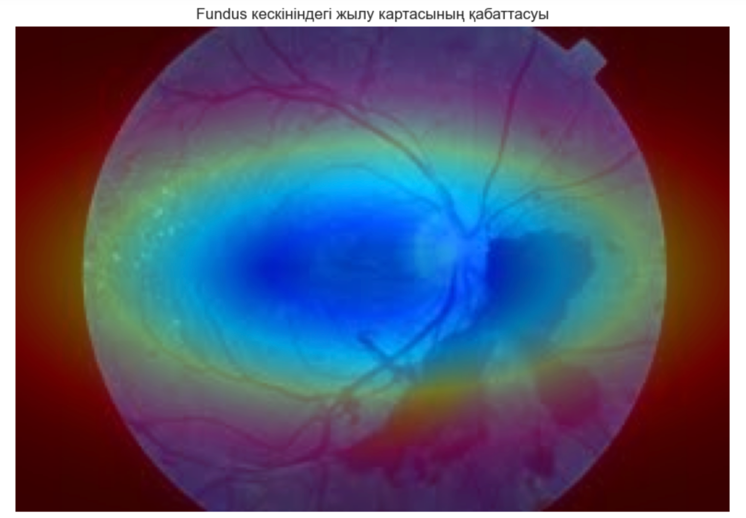
\includegraphics[height=6cm]{media/ict/image20}
		\caption*{1 - сурет. Фундус кескініндегі жылу картасының қабаттасуы}
	\end{subfigure}
	\begin{subfigure}[b]{0.45\textwidth}
		\centering
		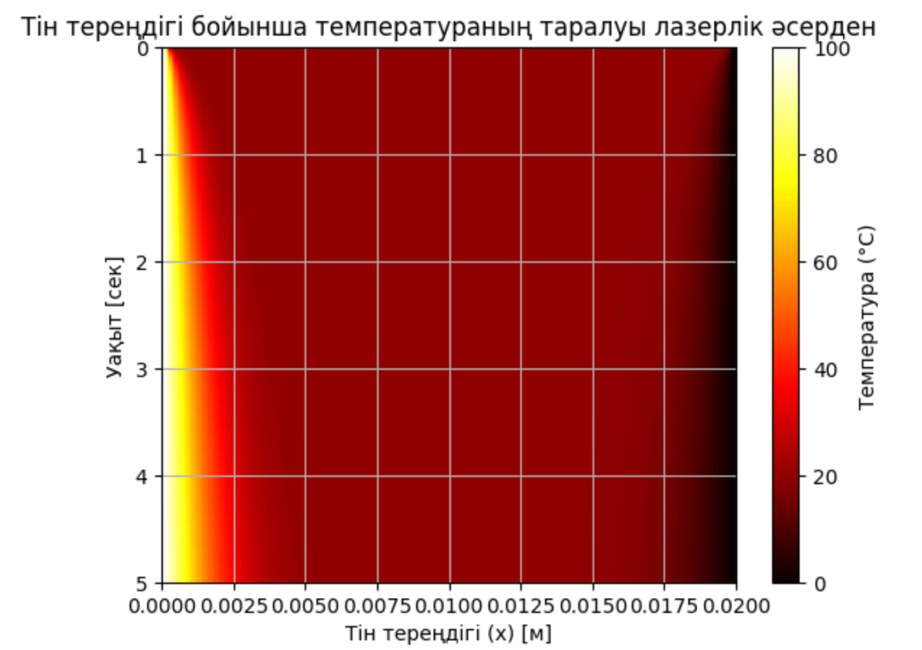
\includegraphics[height=6cm]{media/ict/image21}
		\caption*{2 - сурет. Лазердің әсерінен температураның таралуы}
	\end{subfigure}
\end{figure}

\begin{multicols}{2}
График 2-сурет лазерлік әсерден кейін температураның уақыт пен тереңдік
бойынша таралуын көрсетеді. Х осі тін тереңдігін, Ү осі уақытты, ал
түстер шкаласы температураны көрсетеді. Бұл график лазерлік әсердің
тіндерде таралуын бейнелейді, бұл емдеудің тиімділігін бағалау және
тіндерді артық қыздыру тәуекелін азайту үшін маңызды.
\end{multicols}

\begin{figure}[H]
	\centering
	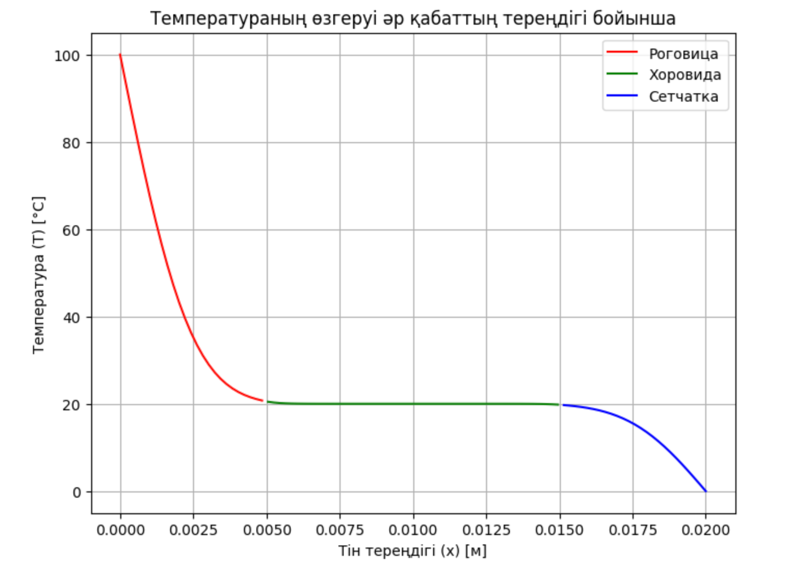
\includegraphics[width=0.6\textwidth]{media/ict/image22}
	\caption*{3 - сурет. Көздің әр қабаты бойынша температураның өзгеруі}
\end{figure}

\begin{multicols}{2}
График тіннің әр қабатындағы температураның тереңдік бойынша өзгеруін
көрсетеді.

- {\bfseries Х осі:} Тін тереңдігі (м), температураның әр қабаттағы
өзгерісін көрсетеді.

- {\bfseries Ү осі:} Температура (градус Цельсиямен), тереңдікке байланысты
температураның өзгеруін көрсетеді.

- {\bfseries Қызы сызық:} Қасаң қабық (роговица), бұл жерде температура
лазерлік энергияның көп сіңірілуіне байланысты тез көтеріледі.

- {\bfseries Жасыл сызық:} Хороид, бұл жерде температураның өзгеруі баяу
жүріп, тұрақты болады.

- {\bfseries Көк сызық:} Көз торы (cетчатка), бұл жерде температура
тереңдікке қарай салыстырмалы түрде тұрақты қалады.
Бұл график 3-сурет лазерлік әсердің тіннің әр қабатына әсерін көрсетеді,
бұл лазерлік параметрлерді оңтайландыру және тіндерді зақымдаудан сақтау
үшін маңызды.
\end{multicols}

\begin{figure}[H]
	\centering
	\begin{subfigure}[b]{0.45\textwidth}
		\centering
		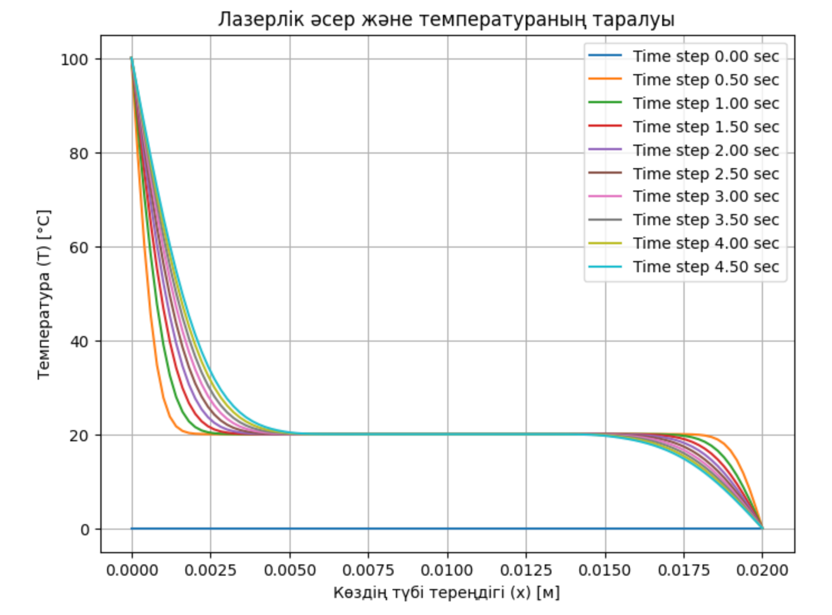
\includegraphics[height=6cm]{media/ict/image23}
		\caption*{4 - сурет. Лазердің әсерінен температураның таралуы}
	\end{subfigure}
	\begin{subfigure}[b]{0.45\textwidth}
		\centering
		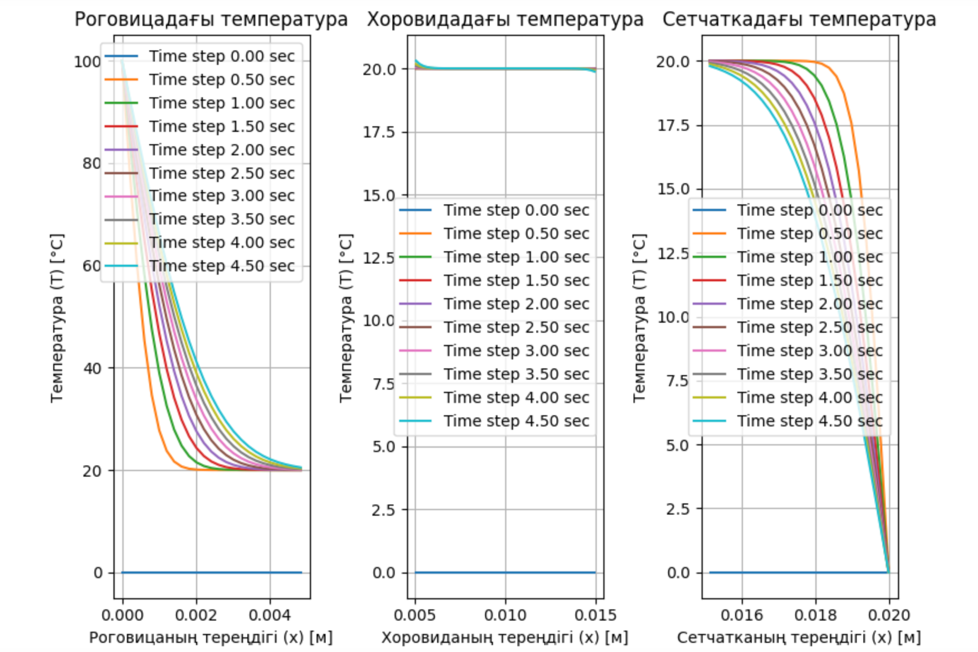
\includegraphics[height=6cm]{media/ict/image24}
		\caption*{5 - сурет. Лазердің әсерінен температураның таралуы}
	\end{subfigure}
\end{figure}

\begin{multicols}{2}
График лазерлік әсер мен температураның таралуын уақыт бойынша
көрсетеді.

- {\bfseries Х осі:} Тін тереңдігі (м), температураның әр түрлі
тереңдіктерде қалай өзгеретінін көрсетеді.

- {\bfseries Ү осі:} Температура (градус Цельсиямен), температураның
өзгеруін көрсетеді.

- {\bfseries Түсті сызықтар:} әр сызық әр уақыт аралығында температураның
өзгеруін көрсетеді (0-ден 4,5 секундқа дейін). Сызықтар уақыт өткен
сайын температураның тіндерінде қалай таралатынын көрсетеді.
Графикте 4-сурет тіннің бетінде температура лазерлік әсерден кейін
бірден артып, кейінірек тереңдікке қарай таралып, уақыт өткен сайын
тұрақтана бастайды. Бұл график лазерлік әсерден кейін температураның
таралу жылдамдығы мен оның ұзақ сақталуын талдауға пайдалы.

Бұл 5-сурет лазердің әр қабаттағы әсерін (роговица, хороида және
сетчатка) тереңдік бойынша уақыт өте келе қалай таралатынын көрсетеді.

- {\bfseries Сол график (Роговица):} Қасаң қабық (роговица) қабатының
тереңдігі бойынша температураның өзгеруін көрсетеді. Уақыт өткен сайын
температура жоғарылайды, кейін тереңдік бойынша біртіндеп таралады.

- {\bfseries Орталық график (Хороид):} Хороид қабатының тереңдігінен
температураның өзгеруі көрсетілген. Бұл қабаттағы температура өзгерісі
баяу болады.

- {\bfseries Оң график (Сетчатка):} Көз торы (cетчатка) қабатындағы
температураның өзгеруі көрсетілген. Бұл қабаттағы температураның
өзгерісі айтарлықтай баяу жүріп, аздап көтеріледі.

Әр графикте уақыт аралығында температураның қалай өзгеретіні көрсетілген
(0 секундтан 4.5 секундқа дейін). Бұл графиктер лазерлік терапияның әр
қабаттағы әсерін визуализациялап, тіндердің әртүрлі қабаттарында
температураның таралуын зерттеуге мүмкіндік береді.

Бұл зерттеуде диабеттік ретинопатияны емдеу мақсатында көздің түбі
тіндеріне лазерлік әсерді модельдеу үшін математикалық модельдер
қолданылды. Нәтижелер көрсеткендей, лазерлік энергия ең көп беткі
қабаттарда, мысалы, қасаң қабықта сіңіріледі, ал терең қабаттарда,
мысалы, көз торында, бұл энергия едәуір төмендейді. Бұл лазердің
параметрлерін (қуаты, импульс ұзақтығы, дақтың диаметрі) дәл баптаудың
дені сау тіндерге зақым келтірмеу үшін қаншалықты маңызды екенің
растайды.

Математикалық модельдер мен жылу карталарын қолдану арқылы көздің түбі
тіндеріндегі температураның уақыт бойынша таралуын талдауға мүмкіндік
береді. Алынған деректер беткі қабаттарда температураның жылдам
көтерілетініне және біршама уақыттан кейін терең қабаттарда
температураның тұрақталатынын көрсетті. Бұл лазерлік әсерді модельдеудің
жоғары деңгейдегі басқаруға қол жеткізуге мүмкіндік беретінін және
тиімді емдеу үшін қажетті қауіпсіздік шараларын қамтамасыз ететінін
дәлелдейді.
\end{multicols}

\begin{figure}[H]
	\centering
	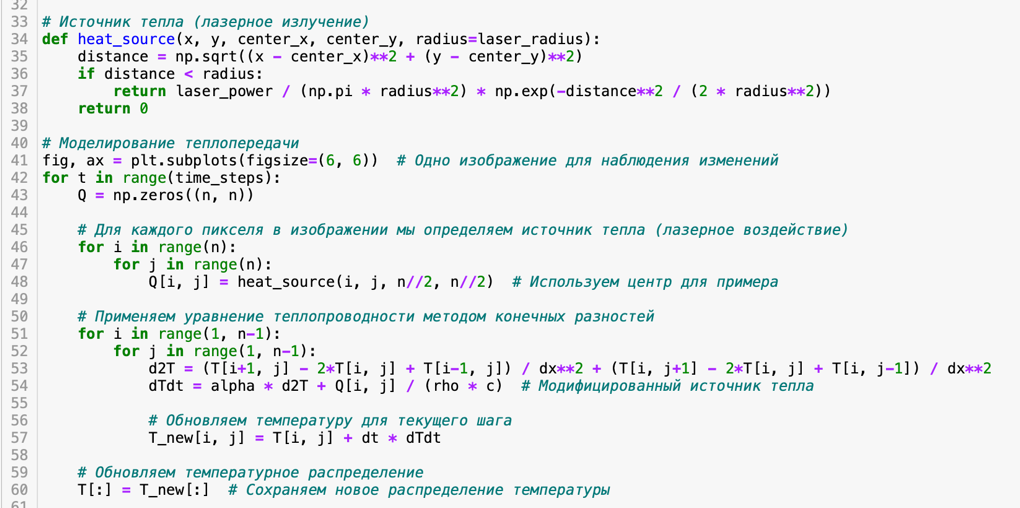
\includegraphics[width=0.8\textwidth]{media/ict/image25}
	\caption*{6 - сурет. Математикалық модельдердің программалық іске асуының көрінісі}
\end{figure}

\begin{multicols}{2}
Ғылыми жұмыстағы математикалық модельді жүзеге асыру және сандық
эксперименттер жүргізу үдерісінде заманауи ақпараттық-коммуникациялық
технологиялар (АКТ) кеңінен қолданылды (6-сурет). Жоғарыда айтылғандай
модельдеу процесі Python бағдарламалау тілінің негізінде құрылып,
есептеу және сандық талдау мақсатында NumPy мен SciPy кітапханалары
пайдаланылды. Температуралық өрістің және лазерлік параметрлердің
кеңістікте таралуын көрнекі түрде бейнелеу үшін Matplotlib және Seaborn
құралдары қолданылды. Зерттеу Jupyter Notebook интерактивті ортасында
жүргізілді, бұл ғылыми есептеулердің құрылымын модульдеу, нәтижелердің
дәлдігін қамтамасыз ету және зерттеу үдерісін қайталамалы етуге
мүмкіндік берді. Осы АКТ құралдарының үйлесімді қолданылуы модельдеу
сапасын арттырып, есептеу нәтижелерін тиімді талдауға және
визуализациялауға жол ашты.

Алдыңғы зерттеулермен салыстырғанда, бұл зерттеудің нәтижелері лазерлік
терапияны қолданудың тиімділігін растайды, бірақ лазер параметрлердің
дәл бапталуының қажеттілігін де айқындайды. Мысалы, авторлардың {[}5{]}
жұмыстарында энергия дозасын дәл есептеу мәселесі көтерілген болатын,
алайда біздің тәсіл көздің түбі тіндеріндегі жылу алмасуды дәл
модельдеуге мүмкіндік береді, бұл клиникалық нәтижелерді жақсартуға
әкелуі мүмкін.

{\bfseries Қорытынды.} Зерттеу нәтижесінде лазерлік терапия үшін
математикалық модель әзірленіп, оның негізінде лазерлік параметрлердің
көздің түбі тіндеріндегі температураға әсерін дәл болжауға мүмкіндік
беретін жүйе жасалды. Жылу әсерлерін модельдеу, оның ішінде
температураның көтерілуі, тіндер энергиясының сіңірілуі және таралуы,
лазерлік емдеудің қауіпсіз әрі тиімді әдістерін жасауға мүмкіндік
береді.

Алынған нәтижелерге сүйене отырып, лазер параметрлерін оңтайландыру дені
сау тіндерге зақым келтірмей, лазерлік әсердің дәлдігі мен тиімділігін
арттыратынын айтуға болады. Бұл офтальмологиядағы лазерлік
технологияларды қолдану мүмкіндіктерін жаңа деңгейге көтеріп, лазерлік
құрылғыларды жасауға негіз болады. Бұл құрылғылар лазерлік энергияны дәл
бағыттай отырып, тек зақымданған аймақтарды емдейді, сау тіндерді
зақымдамайды.

Келешекте жүргізілетін зерттеулер лазерлік энергияның түрлі тіндерге
әсерін тереңірек зерттеп, лазердің көп мәрте қолданылуының ұзақ мерзімді
әсерлерін бағалауға бағытталады.
\end{multicols}

\begin{center}
{\bfseries References}
\end{center}

\begin{references}
1. Shirokanev A., Ilyasova N., Andriyanov N., Zamytskiy E. A., Zolotarev
A., Kirsh D. V. Modeling of Fundus Laser Exposure for Estimating Safe
Laser Coagulation Parameters in the Treatment of Diabetic Retinopathy //
MATH.- 2021. -Vol.9(9).- P.967. DOI 10.3390/MATH9090967.

2. Pashchenko H., Tereshchenko M. Modeling the Impact of Laser
Irradiation on Temperature Changes in Biological Tissues // Vísnik
Kiívskogo Polítéchnícho Instítutu.2024. -№ 67(1).-P.96-102. DOI\\
10.20535/1970.67(1).2024.306876.

3. Chen B., Zhao Y. B., Li D. Numerical Simulation of Ophthalmic Laser
Surgeries by a Local Thermal Non-Equilibrium Two-Temperature Model //
International Journal of Numerical Methods for Heat \& Fluid Flow.-
2019. - Vol.29(12).- P.4706-4723. DOI 10.1108/HFF-05-2019-0397.

4. Mathieu J., Schulmeister K. Validation of a Computer Model to Predict
Laser Induced Retinal Injury Thresholds //Journal of Laser
Applications.- 2017. Vol.29(3).- P.032004. DOI 10.2351/1.4997831.

5. Cvetković M., Poljak D., Peratta A. Thermal Modelling of the Human Eye
Exposed to Laser Radiation // 2008.
\href{https://ieeexplore.ieee.org/xpl/conhome/4662489/proceeding}{16th
International Conference on Software, Telecommunications and Computer
Networks}, P.16-20. DOI 10.1109/SOFTCOM.2008.4669444.

6. Denton M. H., Clark C., Noojin G. D., West H., Stadick A., Khan T.
Unified Modeling of Photothermal and Photochemical Damage // Frontiers
in Ophthalmology.-2024.-Vol.4. DOI 10.3389/fopht.2024.1408869.

7. \href{https://www.researchgate.net/profile/Manuel-Schaller-2?_tp=eyJjb250ZXh0Ijp7ImZpcnN0UGFnZSI6InB1YmxpY2F0aW9uIiwicGFnZSI6InB1YmxpY2F0aW9uIn19}{Schaller}
M. et al. Parameter Estimation and Model Reduction for Retinal Laser
Treatment //// arXiv: Electrical Engineering and Systems Science
\textgreater{} Systems and Control.2022. DOI 10.48550/arxiv.2202.13806.

8. Kotzur S., Wahl S., Frederiksen A. Simulation of Laser Induced Retinal
Thermal Injuries for Non-Uniform Irradiance Profiles and Their
Evaluation According to the Laser Safety Standard // arXiv: Tissues and
Organs.2020. DOI 10.1117/12.2555492.

9. Zheltov G. I., Glazkov V. N., Kirkovsky A. I.,
Podol' tsev A. S. Mathematical Models of Laser/Tissue
Interactions for Treatment and Diagnosis in Ophthalmology // Laser
Applications in Life Sciences.- 1991.-Vol.1403.- P.752-753. DOI
10.1117/12.57371.

10. \href{https://www.researchgate.net/profile/Mario-Cvetkovic?_tp=eyJjb250ZXh0Ijp7ImZpcnN0UGFnZSI6InB1YmxpY2F0aW9uIiwicGFnZSI6InB1YmxpY2F0aW9uIn19}{~Cvetković}
M., Cavka D., Poljak D., Peratta A.3D FEM Temperature Distribution
Analysis of the Human Eye Exposed to Laser Radiation // WIT Transactions
on Engineering Sciences. -2010.- Vol.68.- P.303-312. DOI
10.2495/HT100261.

11. Welch A. J., Priebe L. A., Forster L. D., Gilbert R., Lee C.
Experimental Validation of Thermal Retinal Models of Damage from Laser
Radiation // 1979. DOI 10.21236/ADA074156.

12. Filippov, V. M.~Peripheral retinal laser photocoagulation in the
proactive treatment of proliferative diabetic retinopathy // Russian
Ophthalmology Online.- 2024.-Vol.2(4).-P.221-222.
DOI 10.25276/2312-4911-2024-4-221-222.
\end{references}

\begin{authorinfo}
\emph{{\bfseries Авторлар туралы мәліметтер}}

Сапакова С.З.- ф.-м.ғ.к., қауымдастырылған профессор, «Компьютерлік
инженерия» кафедрасы, Халықаралық ақпараттық технологиялар
университеті,Алматы, Қазақстан, e-mail: sapakovasz@gmail.com;

Есмұхамедов Н. С.- PhD докторанты, «Компьютерлік инженерия» кафедрасы,
Халықаралық ақпараттық технологиялар университеті, Қазақстан, Алматы,
e-mail: yesmukhamedov.yeskendyr@gmail.com;

Даниярова Д.Р. - т.ғ.к., қауымдастырылған профессор, Халықаралық білім
беру корпорациясы, Қазақстан, Алматы, e-mail:~dariia.daniyarova@mail.ru;

Ембердиева А. Б.- ассистент G1, Халықаралық ақпараттық технологиялар
университеті, «Компьютерлік инженерия» кафедрасы, техника ғылымдарының
магистрі, Қазақстан, Алматы,
e-mail: a.yemberdiyeva@iitu.edu.kz;

Арманқызы Р.~-техника ғылымдарының магистрі, Халықаралық ақпараттық
технологиялар университеті, «Компьютерлік инженерия» кафедрасы, лектор,
Қазақстан, Алматы, e-mail:~armankyzyrenata@gmail.com;

Қалдыбаева А. С.- аға оқытушы, «Ақпараттық технологиялар және кітапхана
ісі» кафедрасы, Қазақ ұлттық қыздар педагогикалық университеті,
Қазақста, Алматы, e-mail:~aizhan.seisebek@gmail.com.

\emph{{\bfseries Information about authors}}

Sapakova S. Z.- PhD in Physics and Mathematics, Associate Professor,
Department of Computer Engineering, International University of
Information Technology, Kazakhstan, Almaty, e-mail:
sapakovasz@gmail.com;

Yesmukhamedov N. S.- PhD student, Department of Computer Engineering,
International University of Information Technology, Kazakhstan, e-mail:
yesmukhamedov.yeskendyr@gmail.com;

Daniyarova D.R.- PhD in Technical Sciences, Associate Professor at
International Educational Corporation, Kazakhstan, Almaty, e-mail:
dariia.daniyarova@mail.ru;

Emberdieva A. B.- Assistant G1, International University of Information
Technology, Department of Computer Engineering, Master of Technical
Sciences, Kazakhstan, Almaty, e-mail: a.yemberdiyeva@iitu.edu.kz;

Armankyzy R.-- Master of Technical Sciences, International University of
Information Technology, Department of Computer Engineering, Lecturer,
Kazakhstan, Almaty, e-mail: armankyzyrenata@gmail.com;

Kaldybaeva A. S.- Senior Lecturer, Department of Information Technology
and Library Science, Kazakh National Women' s Pedagogical
University, Kazakhstan, Almaty, e-mail: aizhan.seisebek@gmail.com.
\end{authorinfo}
